\documentclass[12pt,fleqn]{article}\usepackage{../common}
\begin{document}
Coklu Bakis Noktali Geometri (Multiple View Geometry)

[1, sf. 145]

\begin{minted}[fontsize=\footnotesize]{python}
import pandas as pd
import siftpy1
df1 = siftpy1.sift('alcatraz1s.pgm', threshold=10.0)
df2 = siftpy1.sift('alcatraz2s.pgm', threshold=10.0)
\end{minted}

\begin{minted}[fontsize=\footnotesize]{python}
from PIL import Image
im1=Image.open("alcatraz1s.jpg")
im2=Image.open("alcatraz2s.jpg")
df1.plot(kind='scatter',x=0,y=1)
plt.hold(True)
plt.imshow(im1)
plt.savefig('mvg_01.png')
\end{minted}

\begin{minted}[fontsize=\footnotesize]{python}
df2.plot(kind='scatter',x=0,y=1)
plt.hold(True)
plt.imshow(im2)
plt.savefig('mvg_02.png')
\end{minted}


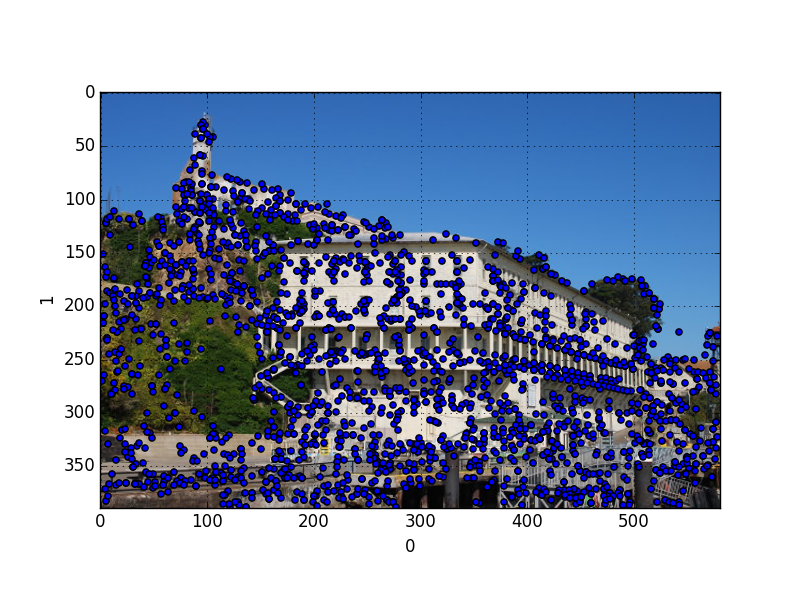
\includegraphics[height=6cm]{mvg_01.png}
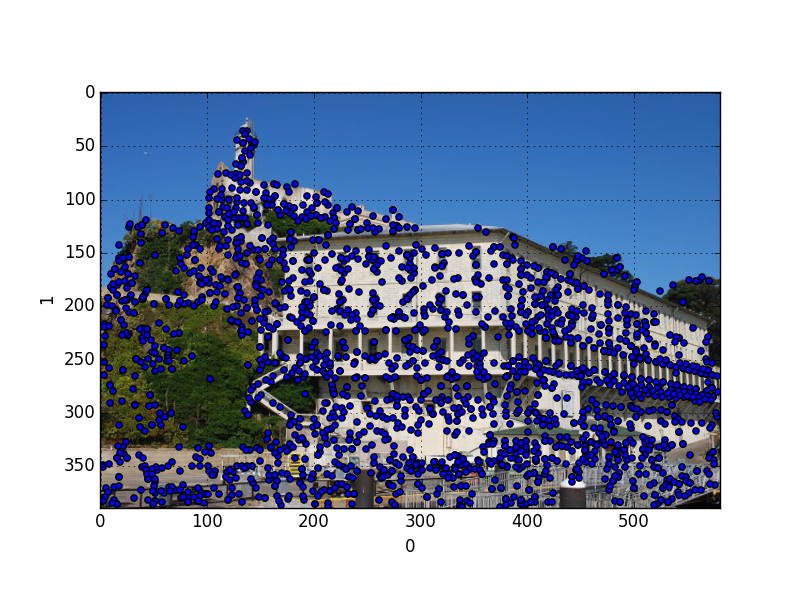
\includegraphics[height=6cm]{mvg_02.png}

\begin{minted}[fontsize=\footnotesize]{python}
matches = siftpy1.match_twosided(df1,df2)
\end{minted}

\begin{minted}[fontsize=\footnotesize]{python}
print matches[:10]
\end{minted}

\begin{verbatim}
[  0 662   1   3   0   0   0   0   0  10]
\end{verbatim}

\begin{minted}[fontsize=\footnotesize]{python}
import homography
import sfm
# calibration
K = np.array([[2394,0,932],[0,2398,628],[0,0,1]])
\end{minted}


\begin{minted}[fontsize=\footnotesize]{python}
import numpy.linalg as lin
l1 = np.array(df1)[:,:4]
l2 = np.array(df2)[:,:4]

ndx = matches.nonzero()[0]
# make homogeneous and normalize with lin.inv(K)
x1 = homography.make_homog(l1[ndx,:2].T)
ndx2 = [int(matches[i]) for i in ndx]
x2 = homography.make_homog(l2[ndx2,:2].T)
x1n = np.dot(lin.inv(K),x1)
x2n = np.dot(lin.inv(K),x2)

# estimate E with RANSAC
model = sfm.RansacModel()
E,inliers = sfm.F_from_ransac(x1n,x2n,model)
\end{minted}

\begin{minted}[fontsize=\footnotesize]{python}
# compute camera matrices (P2 will be list of four solutions)
P1 = np.array([[1,0,0,0],[0,1,0,0],[0,0,1,0]])
P2 = sfm.compute_P_from_essential(E)

# pick the solution with points in front of cameras
ind = 0
maxres = 0
for i in range(4):
    # triangulate inliers and compute depth for each camera
    X = sfm.triangulate(x1n[:,inliers],x2n[:,inliers],P1,P2[i])
    d1 = np.dot(P1,X)[2]
    d2 = np.dot(P2[i],X)[2]
    if np.sum(d1>0)+np.sum(d2>0) > maxres:
        maxres = np.sum(d1>0)+np.sum(d2>0)
        ind = i
        infront = (d1>0) & (d2>0)

# triangulate inliers and remove points not in front of both cameras
X = sfm.triangulate(x1n[:,inliers],x2n[:,inliers],P1,P2[ind])
X = X[:,infront]
\end{minted}


\begin{minted}[fontsize=\footnotesize]{python}
# 3D plot
from mpl_toolkits.mplot3d import axes3d
fig = plt.figure()
ax = fig.gca(projection='3d')
ax.plot(-X[0],X[1],X[2],'k.')
plt.axis('off')
plt.savefig('mvg_03.png')
\end{minted}

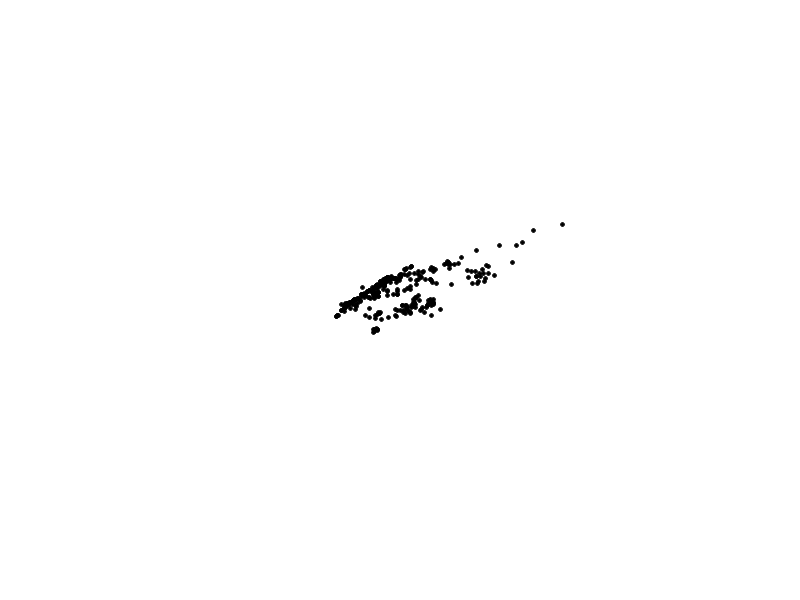
\includegraphics[height=6cm]{mvg_03.png}






















Kaynaklar

[1] Solem, {\em Computer Vision with Python}

\end{document}
